\documentclass[aps,reprint,floatfix]{revtex4-2}

\usepackage{microtype}
\usepackage{fix-cm} % Remove font size substitution warnings
\usepackage{amsmath} % must be loaded before newtxmath
\usepackage{amssymb}
\usepackage{amsthm}
\usepackage{siunitx}
\usepackage{physics}
\usepackage[mathic=true]{mathtools}
\usepackage{graphicx}
\usepackage[usenames,dvipsnames]{xcolor}
\usepackage{tikz}

% \usepackage{etoolbox}
% \makeatletter
% \patchcmd{\section}{\sffamily}{\bfseries}{}{}
% \makeatother

\usepackage[semibold]{libertine} % a bit lighter than Times--no osf in math
\usepackage[libertine,vvarbb]{newtxmath}
\usepackage[scr=esstix,cal=boondoxo]{mathalfa}
\usepackage{bm} % load after all math to give access to bold math
\renewcommand\mathrm\textnormal%

% \allowdisplaybreaks%

\usepackage[pdfusetitle]{hyperref}
\hypersetup{%
  hypertexnames=false, % For compatibility with autonum
  colorlinks,
  allcolors=MidnightBlue,
  citecolor=OliveGreen,
}
\urlstyle{same}
\usepackage{autonum}

\theoremstyle{plain}
\newtheorem{thm}{Theorem}[section]
\newtheorem{lem}{Lemma}
\theoremstyle{definition}
\newtheorem{defn}{Definition}
\newtheorem*{defn*}{Definition}
\newtheorem{post}{Postulate}

\graphicspath{{figs/}}

\usepackage{minted}
\setmonofont[Scale=MatchLowercase]{Iosevka}
\setminted{%
  fontsize=\scriptsize,
  mathescape, style=friendly, baselinestretch=0.9, breaklines
}
\setminted[wolfram]{%
  style=mathematica
}

\renewcommand\leq\leqslant%
\renewcommand\geq\geqslant%

\renewcommand\phi\varphi%


\newcommand\im{\mathrm{i}\mkern1mu}
\renewcommand\ln{\operatorname{\mathrm{ln}}}
\renewcommand\lg{\operatorname{\mathrm{lg}}}
\renewcommand\log{\operatorname{\mathrm{log}}}
\renewcommand\exp{\operatorname{\mathrm{exp}}}
\renewcommand\tr{\operatorname{\mathrm{tr}}}
\renewcommand\det{\operatorname{\mathrm{det}}}

\newcommand\ZZ{\mathbb{Z}}
\newcommand\QQ{\mathbb{Q}}
\newcommand\CC{\mathbb{C}}
\newcommand\RR{\mathbb{R}}

\newcommand{\opr}[1]{\mathsf{#1}}%
\newcommand\idsopr{\mathbb{1}}
\newcommand\idopr{\opr{I}}
\newcommand\sopr\mathcal%
\newcommand\cat\mathsf%
\newcommand\herm{\operatorname{\mathrm{He}}}

% \newcommand\lprod[2]{{\qty(#1,#2)}}
\newcommand\lprod\ip%

\newcommand\hilb{\mathcal{H}}
\newcommand\liou{\mathcal{L}}
\newcommand\ham{\opr{H}}
\newcommand\dop{\opr{ρ}}
\newcommand\tprod\otimes%

\newcommand\ensavg[2][\dop]{\ev{#2}_{\mkern-1.5mu{#1}}}%
\newcommand\sensavg[2][\dop]{\ev*{#2}_{\mkern-1.5mu{#1}}}%

\begin{document}
\title{Understanding visual complexity with statistical physics\\
Rensselaer \textsc{nsf} \textsc{reu} final report}
\author{Alex Striff}
\affiliation{Department of Physics, Reed College, Portland \textsc{or} 97202, \textsc{usa}}
\author{Vincent Meunier}
\affiliation{Department of Physics, Applied Physics, and Astronomy, Rensselaer
Polytechnic Institute, Troy \textsc{ny} 12180, \textsc{usa}}
\date{August 7, 2020}
\begin{abstract}
  An image of natural scene may be described in a few words, yet an image of
  static requires describing all of the pixel values. We call this property of
  images visual complexity. Different perspectives for understanding why natural
  images have low visual complexity have wide applications in fields like
  computer vision and image compression. This \textsc{reu} project reviews
  conventional approaches to visual complexity related to the field of natural
  image statistics, and proposes two new perspectives on visual complexity which
  do not require such statistics: a notion of information for an statistical
  ensemble created by modifying an image, and a notion of how informative
  different coordinate systems are for describing points from a probability
  distribution. Taken together, these different perspectives form a framework
  for understanding visual complexity in a variety of images.
\end{abstract}
\maketitle

{\small
\tableofcontents
}
\newpage

\section{Introduction}

Why is it that thousands of pixels and millions of possible colors are required
to represent images from the natural world on computers, yet that the scene may
be reasonably described as a landscape of a lake at sunset in only these few
words? In more detail, an image is worth a thousand words, yet the file size may
be millions of binary machine words. We call this phenomenon \emph{visual
complexity}. We seek systematic ways to understand the information content or
complexity in images. How are the handful of salient objects present in a scene
related to all of the pixel values captured by a camera, or to the signals in
the brain generated from the eyes? Different notions of visual complexity could
aid progress in fields like computer vision and image compression. For example,
if a computer could render an image from something like a human language
description, file sizes could be much smaller and computer vision tasks like
face recognition or quality control could be improved.

We first define what we mean by information, complexity, and entropy in
Sec.~\ref{sec:bg}. With this backdrop in place, we then look at different
perspectives on visual complexity.

We identify a conventional approach to visual complexity in the literature. This
heap of ideas may be roughly separated into three interconnected perspectives.
We start with the overarching \emph{natural perspective} in
Sec.~\ref{sec:natstat}, which looks at the statistics of images from the natural
world. The \emph{psychophysical perspective} considers the human visual system
in Sec.~\ref{sec:vision}. Finally, we look past data on lattices like the fovea
or sets of pixels, and instead hold the processes that create the data to be
responsible for their complexity. The \emph{algorithmic perspective} of
Sec.~\ref{sec:graphics} considers programs as explanations of complexity, with
commonly-used computer graphics techniques serving as upper bounds on the true
algorithmic complexity.

We propose a new perspective on the information content of an image modification
that is inspired by statistical physics. To this end, we propose an ensemble of
images that are different from a given image in Sec.~\ref{sec:wl}. This
\emph{ensemble perspective} considers the information to describe the
modification to be much like the information to specify a microstate in
statistical physics. The natural and ensemble perspectives usually work with
grayscale images. The complications associated with considering color arise from
the choice of coordinates for the color space. This is addressed by the
\emph{coordinate perspective} that we propose in Sec.~\ref{sec:color}. All of
these perspectives contribute to defining the notion of visual complexity.

\section{Information, Entropy, and Complexity}\label{sec:bg}

We generally use these terms as synonyms for the same kind of idea, but with
different connotations from information theory, statistical physics, and
computer science, respectively.

\subsection{Information Theory}\label{sec:information-theory}

A mathematical notion of information is provided by the work of
Shannon~\cite{shannon1948mathematical}. In the view of classical information
theory, \emph{information} is a property of an event, in the sense of a random
process. To this end, we consider a random variable $X$ with support
$\mathcal{X}$ and probabilities $p(x)$ for $x \in \mathcal{X}$. As regards
communication, the information $I(x)$ required to describe the event $X = x$
should satisfy intuitive axioms:
\begin{itemize}
  \item If $p(x) = 1$, the event is certain to happen and no information is
    required to describe its occurrence: $I(x) = 0$.
  \item If $p(x) < p(x')$, then $x$ is less likely to happen, and ought to
    require more information to describe: $I(x) > I(x') \geq 0$. As an analogy,
    compare the phrases ``nightly'' and ``once in a full moon:'' The less
    probable event has a longer description.
  \item For independent events $x$ and $y$, it makes no difference to describe
    the combined event $(x,\, y)$ instead of each event individually: $I(x,\, y)
    = I(x) + I(y)$.
\end{itemize}

Given these axioms, the only solution is the
\emph{self-information}~(Theorem~\ref{thm:self-information})
\begin{equation}
  I(x)
  = -\log p(x),
  \label{eq:self-information}
\end{equation}
where the base of the logarithm determines the units of information: base two
($\lg$) gives \emph{bits} and base $e$ ($\ln$) gives \emph{nats}. The
information of the entire random variable may then be defined as the average
of~\eqref{eq:self-information} over all events, which is known as the
\emph{Shannon entropy}
\begin{equation}
  H
  = -\sum_{x \in \mathcal{X}} p(x) \log p(x).
  \label{eq:shannon-entropy}
\end{equation}
The Shannon entropy may also be derived from intuitive axioms similar to those
for the self information~\cite{shannon1948mathematical,jaynes1957information}.
The continuous version of~\eqref{eq:shannon-entropy} is known as the
\emph{differential entropy}
\begin{equation}
  h
  = -\int_{\mathcal{X}} p(x) \log p(x) \dd{x},
  \label{eq:differential-entropy}
\end{equation}
which is insufficient as a notion of information because it may change with
different coordinates. Instead, we consider the \emph{relative entropy} or
\emph{Kullback-Leibler divergence} from a reference distribution $q$ to $p$
defined by
\begin{equation}
  D_{KL}(p \mathbin{\|} q)
  = \int_{\mathcal{X}} p(x) \log \frac{p(x)}{q(x)} \dd{x},
  \label{eq:kl-divergence}
\end{equation}
which is invariant under parameter transformations and
is nonnegative~\cite[p.~243]{cover}.

\subsection{The maximum entropy principle (\textsc{MaxEnt})}\label{sec:maxent}

A physicist familiar with statistical mechanics might wonder why Shannon's
entropy~\eqref{eq:shannon-entropy} has the same mathematical form as the
thermodynamic state variable for temperature
\begin{equation}
  S
  = -k_B \sum_{x \in \mathcal{X}} p(x) \ln p(x),
  \label{eq:gibbs-entropy}
\end{equation}
which we may call the \emph{Gibbs entropy}. This connection between information
theory and statistical physics was developed by E. T. Jaynes to produce the
maximum entropy principle (\textsc{MaxEnt})~\cite{jaynes1957information}. We
would like to make predictions about systems given some macroscopic quantities
that we observe. To do so, we must assign probabilities to microstates, which we
ought to do in an unbiased way, subject to the constraints that average
macroscopic quantities take their observed values. Jaynes argues that this
unbiased assignment corresponds to maximizing the entropy, and describes how
this subjective assignment can be expected to make physical predictions, while
an objective assignment of probabilities is required to understand the
microscopic mechanisms behind these predictions. In particular, maximizing the
entropy with constrained average energy produces the canonical
distribution~\cite{jaynes1957information}
\[
  p(x)
  = \frac{1}{Z}e^{-\beta E(x)},
\]
where $\beta = \flatfrac{1}{k_B T}$ and the \emph{partition function} is
\[
  Z
  = \sum_{x \in \mathcal{X}} e^{-\beta E(x)},
\]
with the variates $x$ being different states of a system.

\subsection{Algorithmic entropy}

A more general notion of entropy is found in an algorithmic approach. We say a
\emph{computer} takes a finite binary string $p \in \qty{0,\, 1}^*$ called a
\emph{program}, and either produces a finite string as output or produces an
infinite string and does not halt.
\begin{defn*}\label{def:kolmogorov}
  Given an object $x$ (representable as a binary string), its \emph{Kolmogorov
  complexity} $K(x)$ is defined as the length of the shortest program that
  outputs the object when executed on a computer.
\end{defn*}
The canonical choice of computer is a universal Turing machine $\mathcal{U}$,
but the complexity from different computer $\mathcal{A}$ (like a Python
interpreter) differs by only a constant: $K_{\mathcal{U}}(x) \leq
K_{\mathcal{A}}(x) + c_{\mathcal{A}}$~\cite[p.~467]{cover}. That is, the
universal computer $\mathcal{U}$ may compute $x$ by simulating $\mathcal{A}$.
For long strings $x$, the constant is insignificant. We may also define the
\emph{conditional Kolmogorov complexity} $K(x \mathbin{|} l(x))$, where the
computer already knows the length of $x$.

The generality of Kolmogorov complexity is apparent when we consider stochastic
processes. Similar to in Sec.~\ref{sec:information-theory}, consider a
stochastic process $\qty{X_i}$ with the $X_i$ drawn \textsc{iid} from the finite set
$\mathcal{X}$ with \textsc{pmf} $p(x)$ for $x \in \mathcal{X}$.
Then~\cite[p.~473]{cover}
\begin{equation}
  H(X)
  = \lim_{n \to \infty} \frac{1}{n}\ev{K(X^n \mathbin{|} n)}.
  \label{eq:complexity-entropy}
\end{equation}
The length of an optimal compression program approaches the entropy limit. In
this sense, the Kolmogorov complexity is a generalization of entropy.

In practice, we do not use minimum-length programs or know Kolmogorov
complexities, since in general they are not computable~\cite[p.~482]{cover}.
However, they are useful in applications of Occam's razor. To avoid multiplying
our explanations beyond necessity, we choose the least complex explanation that
is correct.

\section{Natural image statistics}\label{sec:natstat}

Images of the natural world are easily distinguishable from man-made images or
random noise. This difference is reflected in the statistical structure of
natural images, and is generally robust across variations in subject matter or
lighting. For example, the power spectrum of a natural image (averaged over
orientations), scales like $k^{-2 + \eta}$, where $k$ is the spatial frequency
and $\eta$ is small. This and the other statistics discussed in~\cite{ruderman}
establish that natural images are approximately \emph{scale-invariant}. The
scale invariance of natural images is mostly explained by
occlusion~\cite{dead-leaves}. Different objects appear to be different sizes and
occlude one another, causing an image to depict multiple scales. However, the
scale invariance of a natural image may also reflect the scale invariance of
objects it depicts: nature is full of fractals~\cite{fractals-everywhere}.

\section{Human vision}\label{sec:vision}

The psychophysical perspective on visual complexity focuses on the light
entering the eye and the various responses generated in different regions of the
brain.

\subsection{The light field}\label{sec:light-field}

We may describe the light field from a scene impinging upon the eye with the
\emph{plenoptic function} $L$. This function gives the spectral radiance of
light with wavelength $\lambda$ along a ray specified by spherical angles
$\theta$ and $\phi$ at a given point $(\bm{x},\, t)$ in space and time. All of
the information about how a scene looks is contained in the function
$L(\bm{x},\, t,\, \theta,\, \phi,\, \lambda)$. The creation of \emph{light field
cameras} to capture the whole light field that would enter the eye is a topic
of active research~\cite{light-field}. While our eyes and conventional cameras
use many photosensitive elements, significant capture of the light field may be
done with only one intensity-sensitive element. This is simple enough that the
author previously created a proof of concept \emph{single-pixel camera} for an
undergraduate laboratory project~\cite{csjlab,single-pixel}. Such a
\emph{single-pixel camera} and advances in light-field cameras are made feasible
by a \emph{compressive sensing} technique which leverages the power-law
statistics of natural images discussed in
Sec.~\ref{sec:natstat}~\cite{compressed-sensing}.

\subsection{The visual system}\label{sec:visual-system}

The early stages of processing in the visual system recognize local properties
like color, edge orientation, motion, and binocular disparity. These properties
arise naturally from the plenoptic function, as discussed in~\cite{plenoptic}.
More precisely, one may show simple images to an animal and probe the responses
of neurons in affected regions of the brain, like the lateral geniculate nucleus
(\textsc{lgn}) and primary visual cortex (\textsc{v1}). By varying the stimulus,
one may develop a map of how the neuron responds as a function of position in
$\theta$ and $\phi$. This map, called the \emph{receptive field} of the neuron,
is generally set up to capture an aspect of the plenoptic function. For example,
the receptive fields of \emph{simple cells} in \textsc{v1} are similar to Gabor
filters, and are used to detect edges with a particular
orientation~\cite{plenoptic}. Van Hateren and Ruderman have shown that the
independent components of natural image sequences give similarly shaped filters,
supporting the hypothesis that the simple cell receptive fields are tuned to
encode natural images well~\cite{strf}.

\section{Algorithmic complexity of natural images}\label{sec:graphics}

The computer renderings of natural scenes that are widely used in media can be
convincing to the eye without needing to simulate or model the scene at a
physical level of detail. The low algorithmic complexity of a rendering
reflects the low algorithmic complexity of aspects of a natural scene. In
computer graphics, one usually manipulates the \emph{geometry} of objects and
the \emph{textures} drawn on the geometry. Both of these aspects of a model can
have low complexities.

\subsection{Geometry}

While most geometry in a scene is manually modeled, some natural objects like
trees can be generated algorithmically. The first comprehensive approach was
through the \emph{Lindenmayer systems} studied in \textit{The Algorithmic Beauty
of Plants}~\cite{lindenmayer}. This and other techniques are used in the
commercial \emph{SpeedTree} software package, which is widely used for movies
and video games~\cite{speedtree}. Another technique is to use naturalistic
power-law noise to generate terrain and other structures. The most common
implementation is to combine band-limited noise at different scales, where the
noise is either Perlin or simplex noise~\cite{perlin}.

\subsection{Texture}

Realistic textures may also be synthesized from noise, and further improvement
in realism is found from applying nonlinear transformations and turbulence to a
noise texture~\cite{perlin, hypertexture}. Repeating patterns like tile or
weaves are also simple to generate.

\subsection{Fractals: between geometry and texture}

More aspects of the natural world may be described by fractals. A more detailed
account of these ideas and how they relate to natural images may be found in
\textit{The Science of Fractal Images}~\cite{scifract}. An application of these
ideas is the use of \emph{iterated function systems} (\textsc{ifs}es) to
compress natural images by taking advantage of their
self-similarity~\cite[p.~228]{scifract}. This technique can achieve compression
ratios that are superior to those of common formats like \textsc{jpeg}, at the
cost of being asymmetric. Compression by finding an \textsc{ifs} representation
can take a long time, but the decompression by simulating the \textsc{ifs} is
fast.

\section{An ensemble of images}\label{sec:wl}

We now neglect the spatial structure of natural image statistics and consider
digital images as collections of pixels. We would like to know the information needed to
specify a modification or fluctuation of the pixel values, given that the magnitude of the
modification is approximately known.

\subsection{Theory}\label{sec:wl-theory}

\begin{figure}
  \centering
  \tikzstyle{emph} = [fill=MidnightBlue]
  \begin{tikzpicture}[scale=0.5]%, every node/.style={transform shape}]
    \node[left] at (1.25*1, 1 + 0.5) {\small$1$};
    \node[left] at (1.25*1, 5 + 0.5) {\small$M$};
    \node[below] at (1.25*1 + 0.5,1) {\small$1$};
    \node[below] at (1.25*4 + 0.5,1) {\small$N$};
    \fill[gray] (1.25*1,4) rectangle ++(1,1);
    \fill[emph] (1.25*1,3) rectangle ++(1,1);
    \fill[gray] (1.25*2,1) rectangle ++(1,1);
    \fill[emph] (1.25*2,5) rectangle ++(1,1);
    \fill[gray] (1.25*4,2) rectangle ++(1,1);
    \fill[emph] (1.25*4,4) rectangle ++(1,1);
    \draw[emph] (1.25*4 + 1, 2 + 0.5) -- ++(0.75,0);
    \draw[emph] (1.25*4 + 1, 4 + 0.5) -- ++(0.75,0);
    \draw[emph,<->,thick] (1.25*4 + 1.5, 2 + 0.5) -- ++(0,2)
      node[midway,right]{$\Delta E_N = 2$};
    \node (ellipses) at (1.25*3 + 0.5, 3 + 0.5) {$\cdots$};
    \foreach \x in {1,2,4} {%
      \foreach \y in {1,...,5} {%
        \draw (1.25*\x,\y) rectangle ++(1,1);
      }
    }
  \end{tikzpicture}
  \caption{The energy difference between base image pixel values
    (\textcolor{gray}{$\blacksquare$}) and modified image pixel values
    (\textcolor{MidnightBlue}{$\blacksquare$}).
  }\label{fig:image-levels}
\end{figure}

Given a base image $A$ with $N$ pixels which take integer gray values $1 \leq
a_i \leq M$, we define the \emph{energy} of a different image $B$ with gray
values $1 \leq b_i \leq M$ as
\begin{equation}
  E_A(B)
  = \sum_{i=1}^N \abs{a_i - b_i},
  \label{eq:energy}
\end{equation}
as depicted in Fig.~\ref{fig:image-levels}.

We would like to consider all possible modified images, but focus on images with
a typical value for the energy which indicates the size of fluctuations we are
considering. We do this by assigning a probability distribution to the images
with constrained average energy. Given the results of Sec.~\ref{sec:maxent}, we
choose the \textsc{MaxEnt} distribution, which we may consider as a canonical
ensemble. By thinking of our images as a physical system, we may apply tools
from statistical mechanics. We would like to know the entropy of the
\textsc{MaxEnt} distribution, which we will compute with the partition function as
\begin{equation}
  \flatfrac{S}{k_B}
  = \beta E + \ln Z.
  \label{eq:canonical-entropy}
\end{equation}
In turn, we obtain the partition function
\begin{equation}
  Z
  = \sum_{E \in E(\mathcal{X})} g(E) e^{-\beta E}
  \label{eq:partition-function}
\end{equation}
from the number of states $g(E)$ with energy $E$ (the \emph{density of states}).
For the case where the base image is all black ($a_i = 1$) or all white ($a_i =
M$), we may explicitly count that the density of states
is~(Theorem~\ref{thm:bw-g})
\begin{equation}
  g(E;\, N,\, M)
  = \sum_k {(-1)}^k \binom{N}{k} \binom{N + E - Mk - 1}{E - Mk}.
  \label{eq:bw-g}
\end{equation}
However, the situation for general grayscale images becomes more complicated.
For this reason and the ability to analyze more complex systems, we determine
the density of states numerically using the Wang-Landau
algorithm~\cite{wanglandau}.

\subsection{Methods}\label{sec:wl-methods}

The Wang-Landau algorithm (WL) was implemented to determine the density of
states for grayscale image fluctuations. Our implementation adapts the algorithm
described by Wang, Landau, et al.\ in~\cite{wanglandau,wanglandau-ajp} for
lattice models to work on the image fluctuation model we have described
(Appendix~\ref{sec:wanglandau-core}). The offset of the log density of states
was set by ensuring that the number of states from $\sum_E g(E)$ gave the total
number of states $M^N$. We then computed the entropy from the numerical density
of states with~\eqref{eq:canonical-entropy}.

\subsection{Results}\label{sec:wl-results}

\begin{figure}
  \centering
  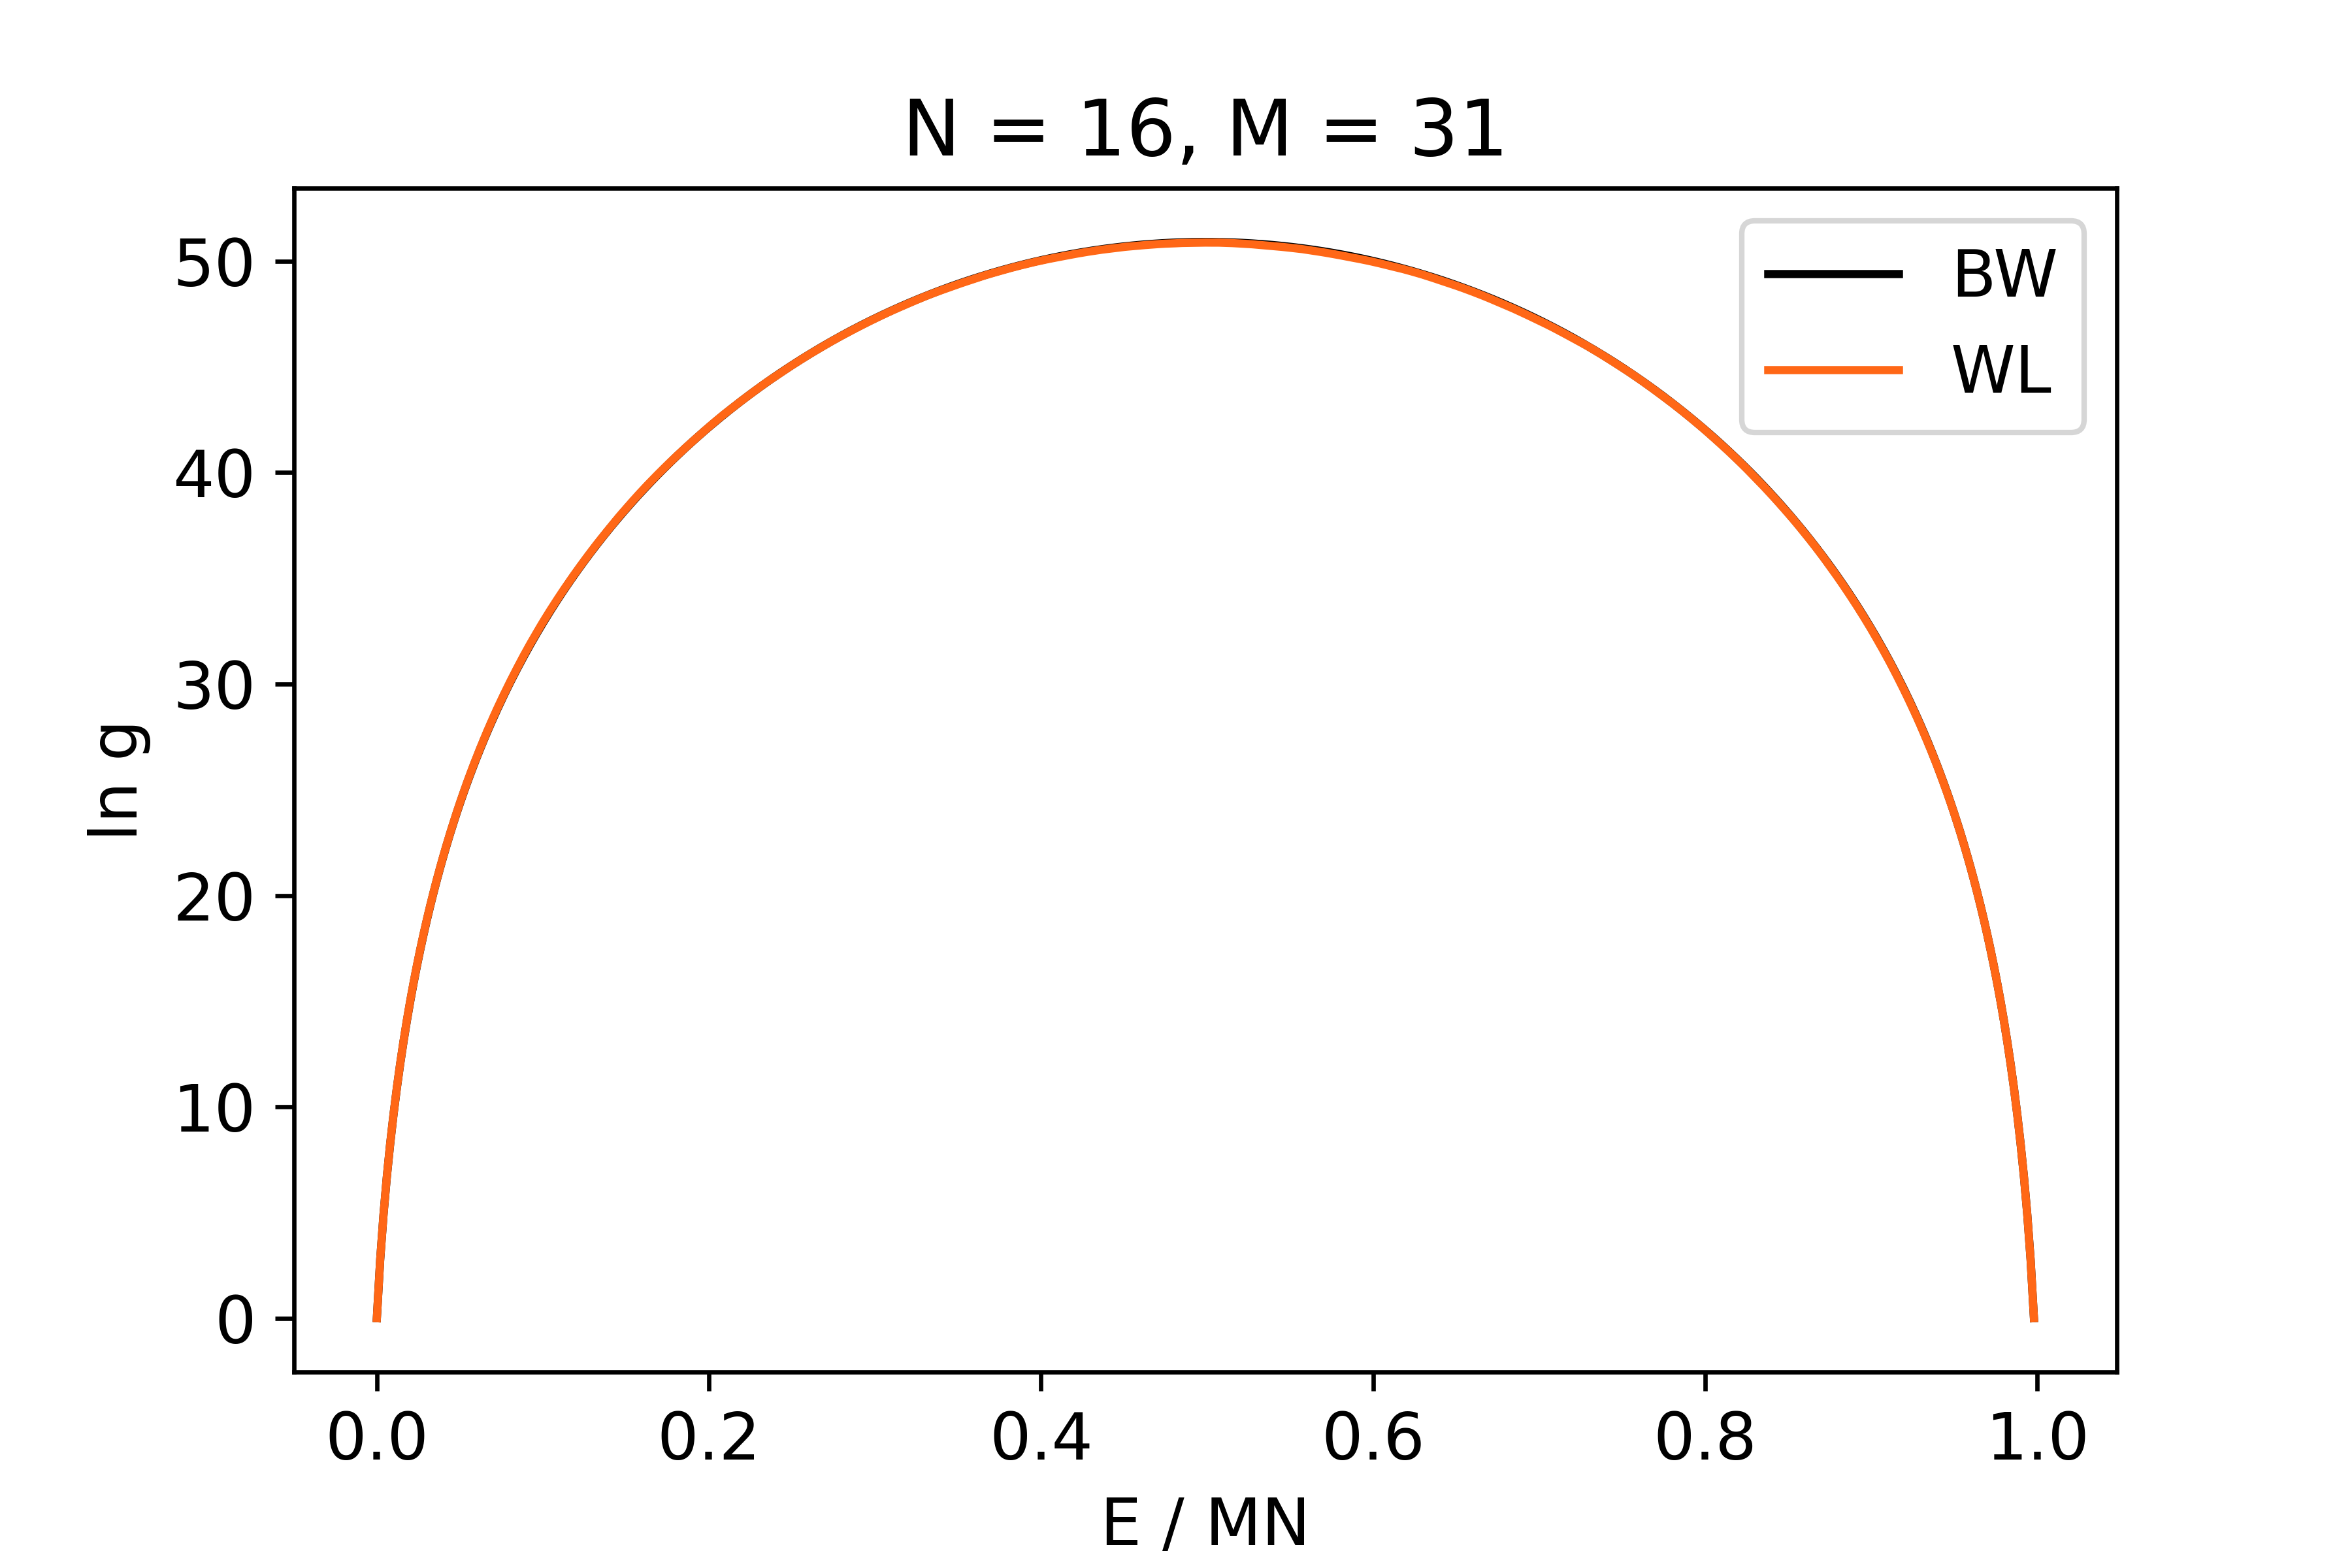
\includegraphics[width=\linewidth]{wanglandau-bw}
  \caption{The log density of states for a black image from the Wang-Landau
    algorithm (WL), compared to the exact result (BW). The two densities of
  states are indistinguishable.}\label{fig:wl-bw}
\end{figure}

\begin{figure}
  \centering
  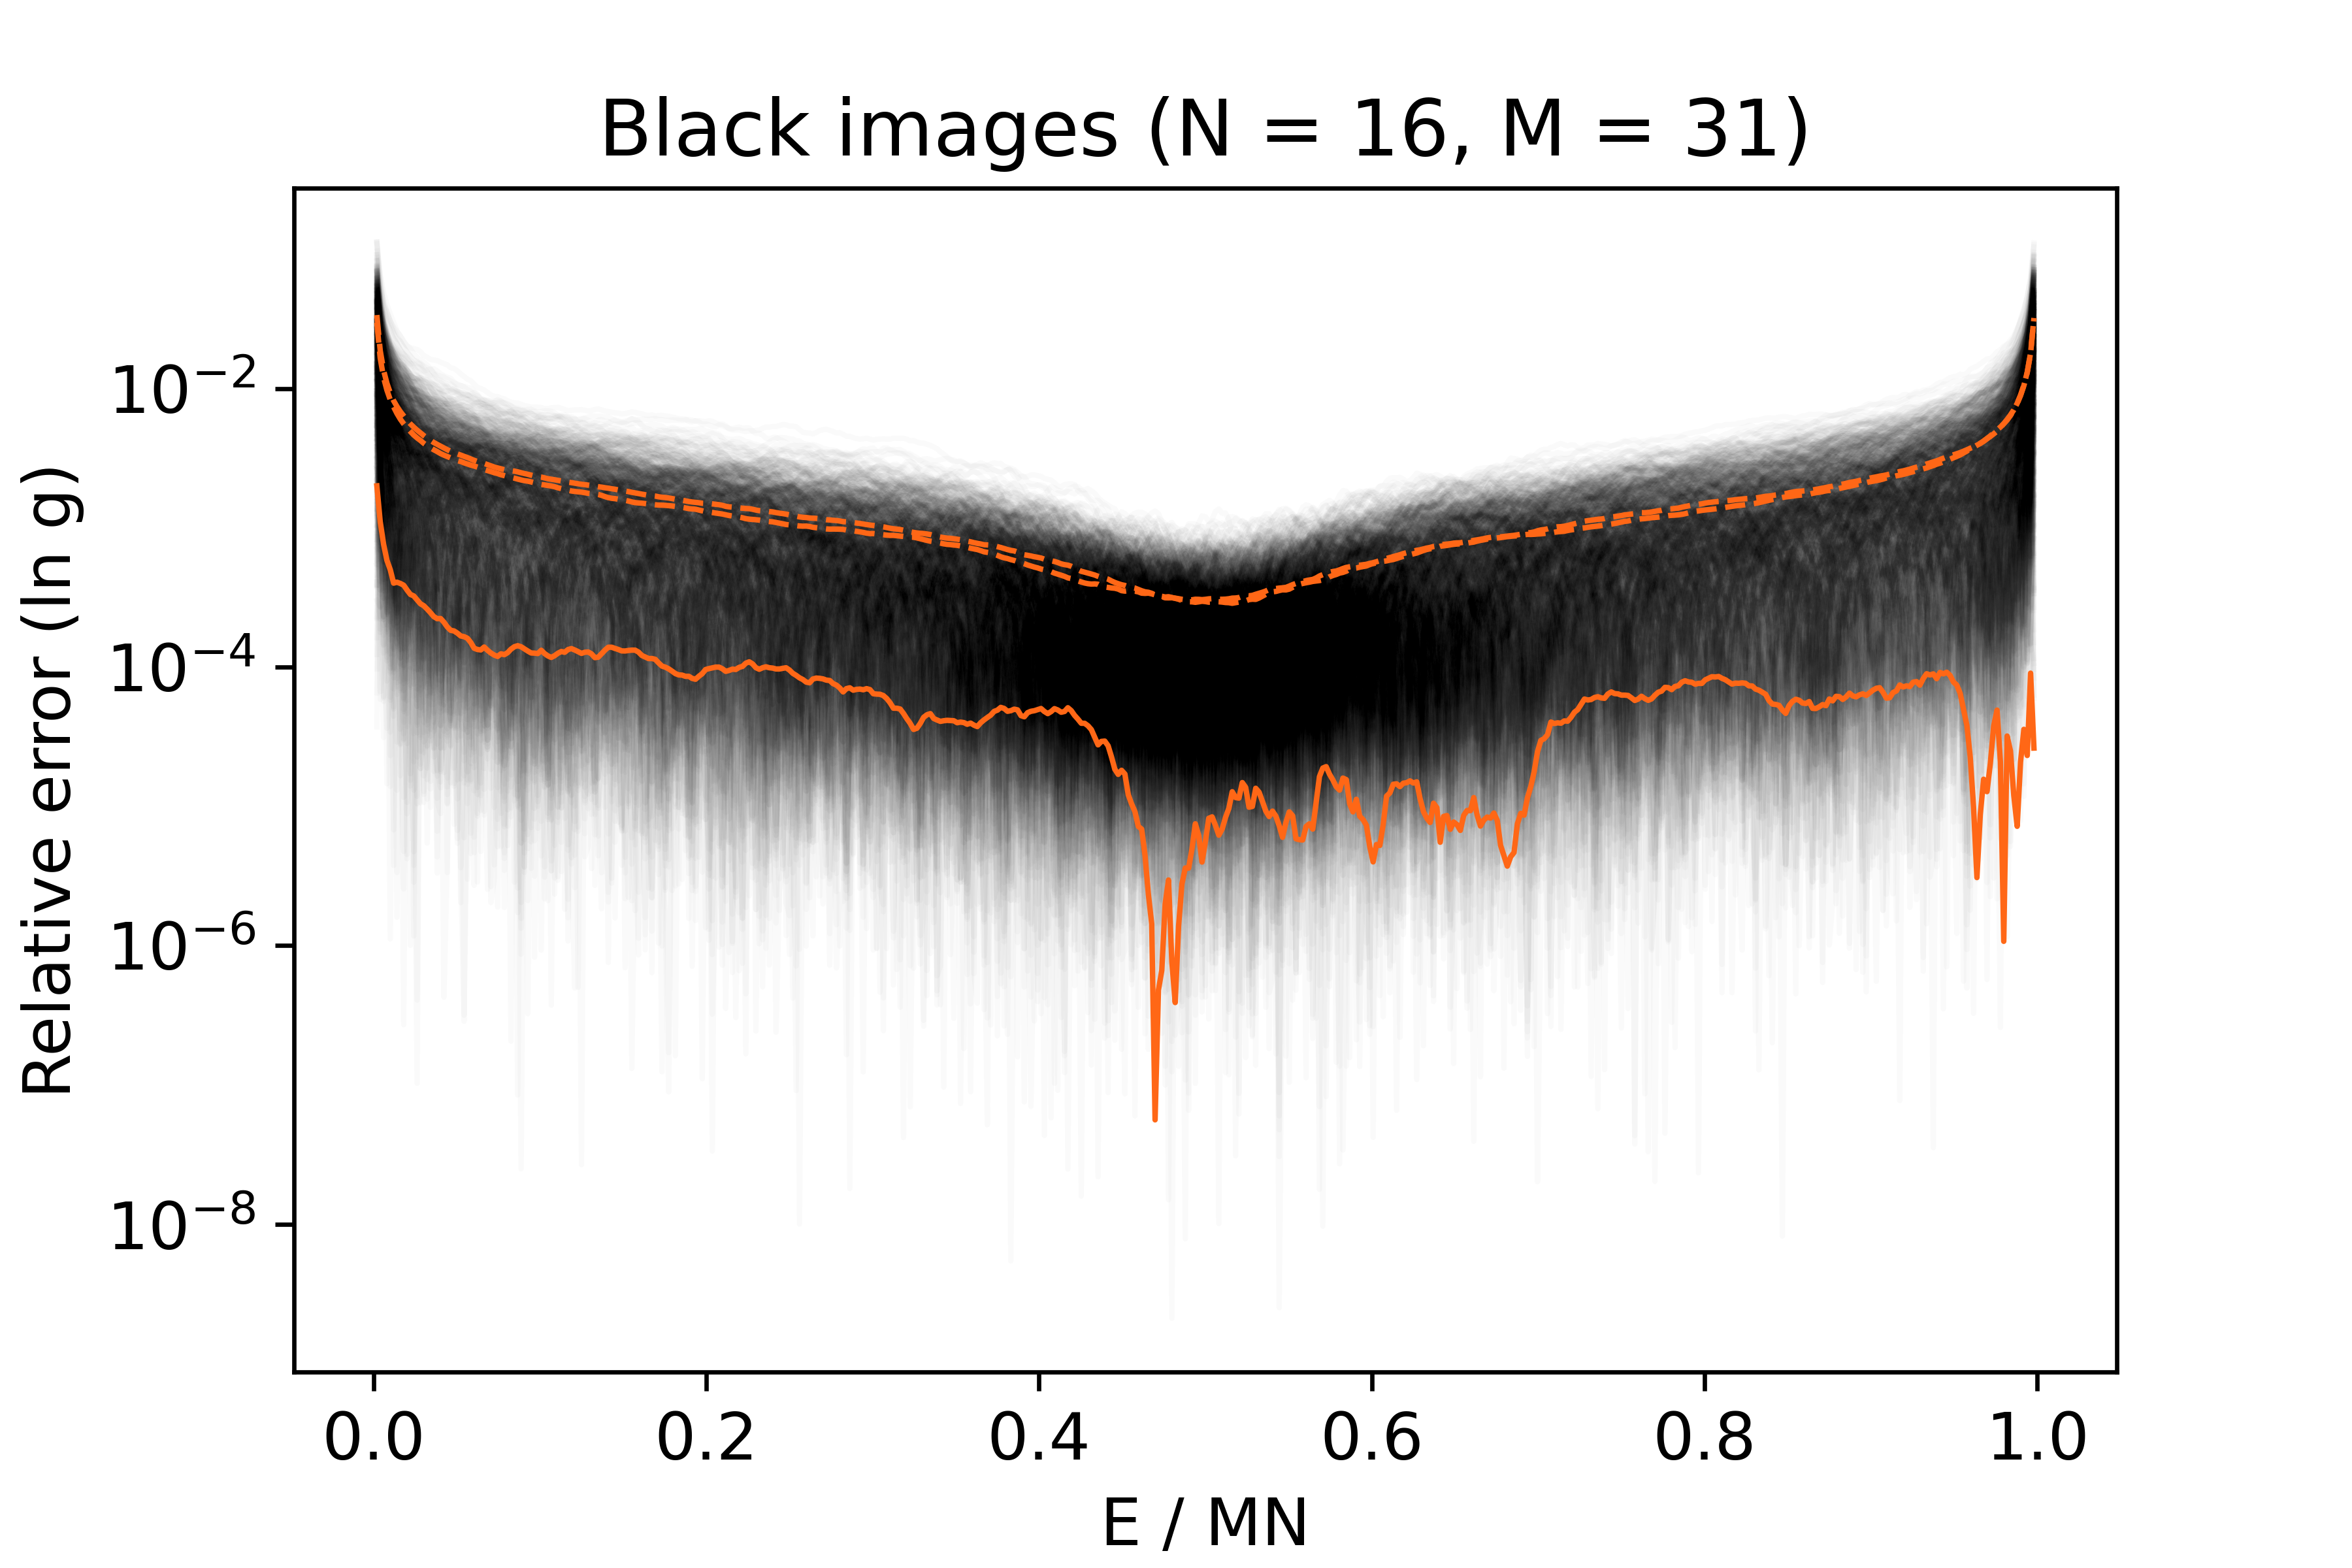
\includegraphics[width=\linewidth]{wanglandau-bw-relerror}
  \caption{The relative error in the log density of states for \num{1024} black
    image Wang-Landau simulations. The mean density of states is indicated
    in orange and the composite densities of states one standard deviation away
  are dashed.}\label{fig:wl-bw-relerror}
\end{figure}

\begin{figure}
  \centering
  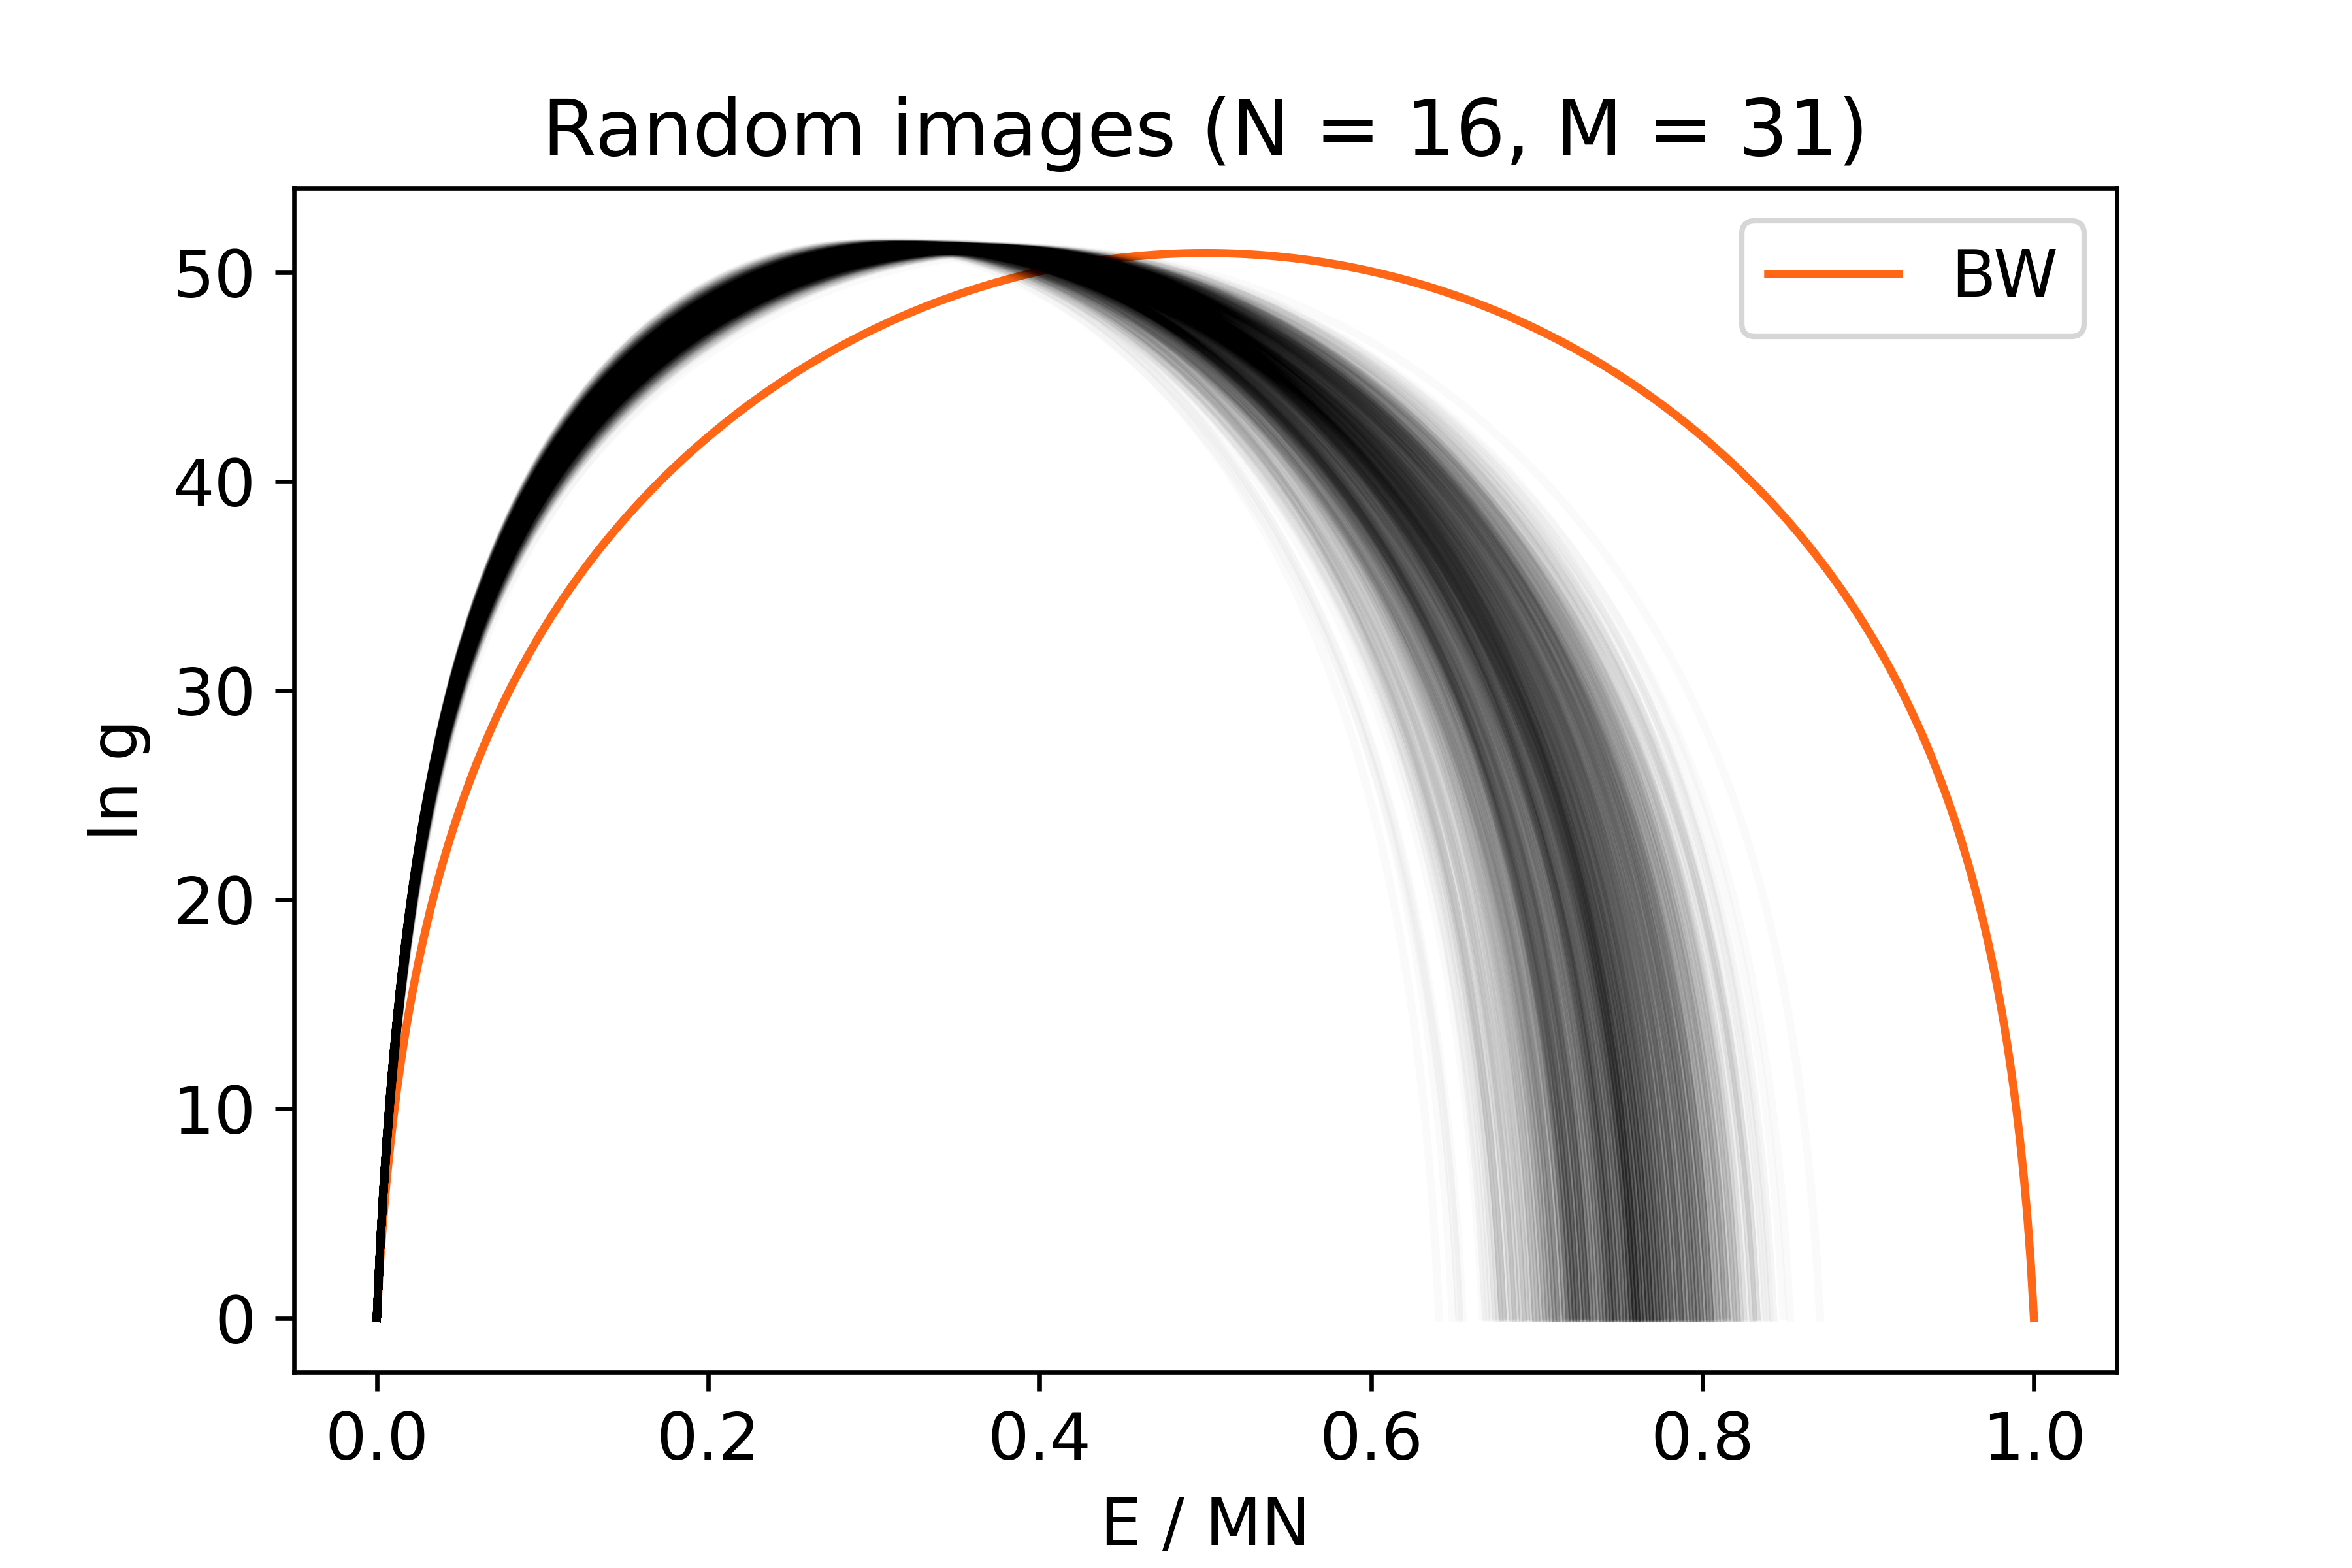
\includegraphics[width=\linewidth]{wanglandau-gray}
  \caption{The log density of states for \num{1024} random grayscale image
    Wang-Landau simulations. The black image result is provided as
  reference in orange (BW).}\label{fig:wl-gray}
\end{figure}

\begin{figure}
  \centering
  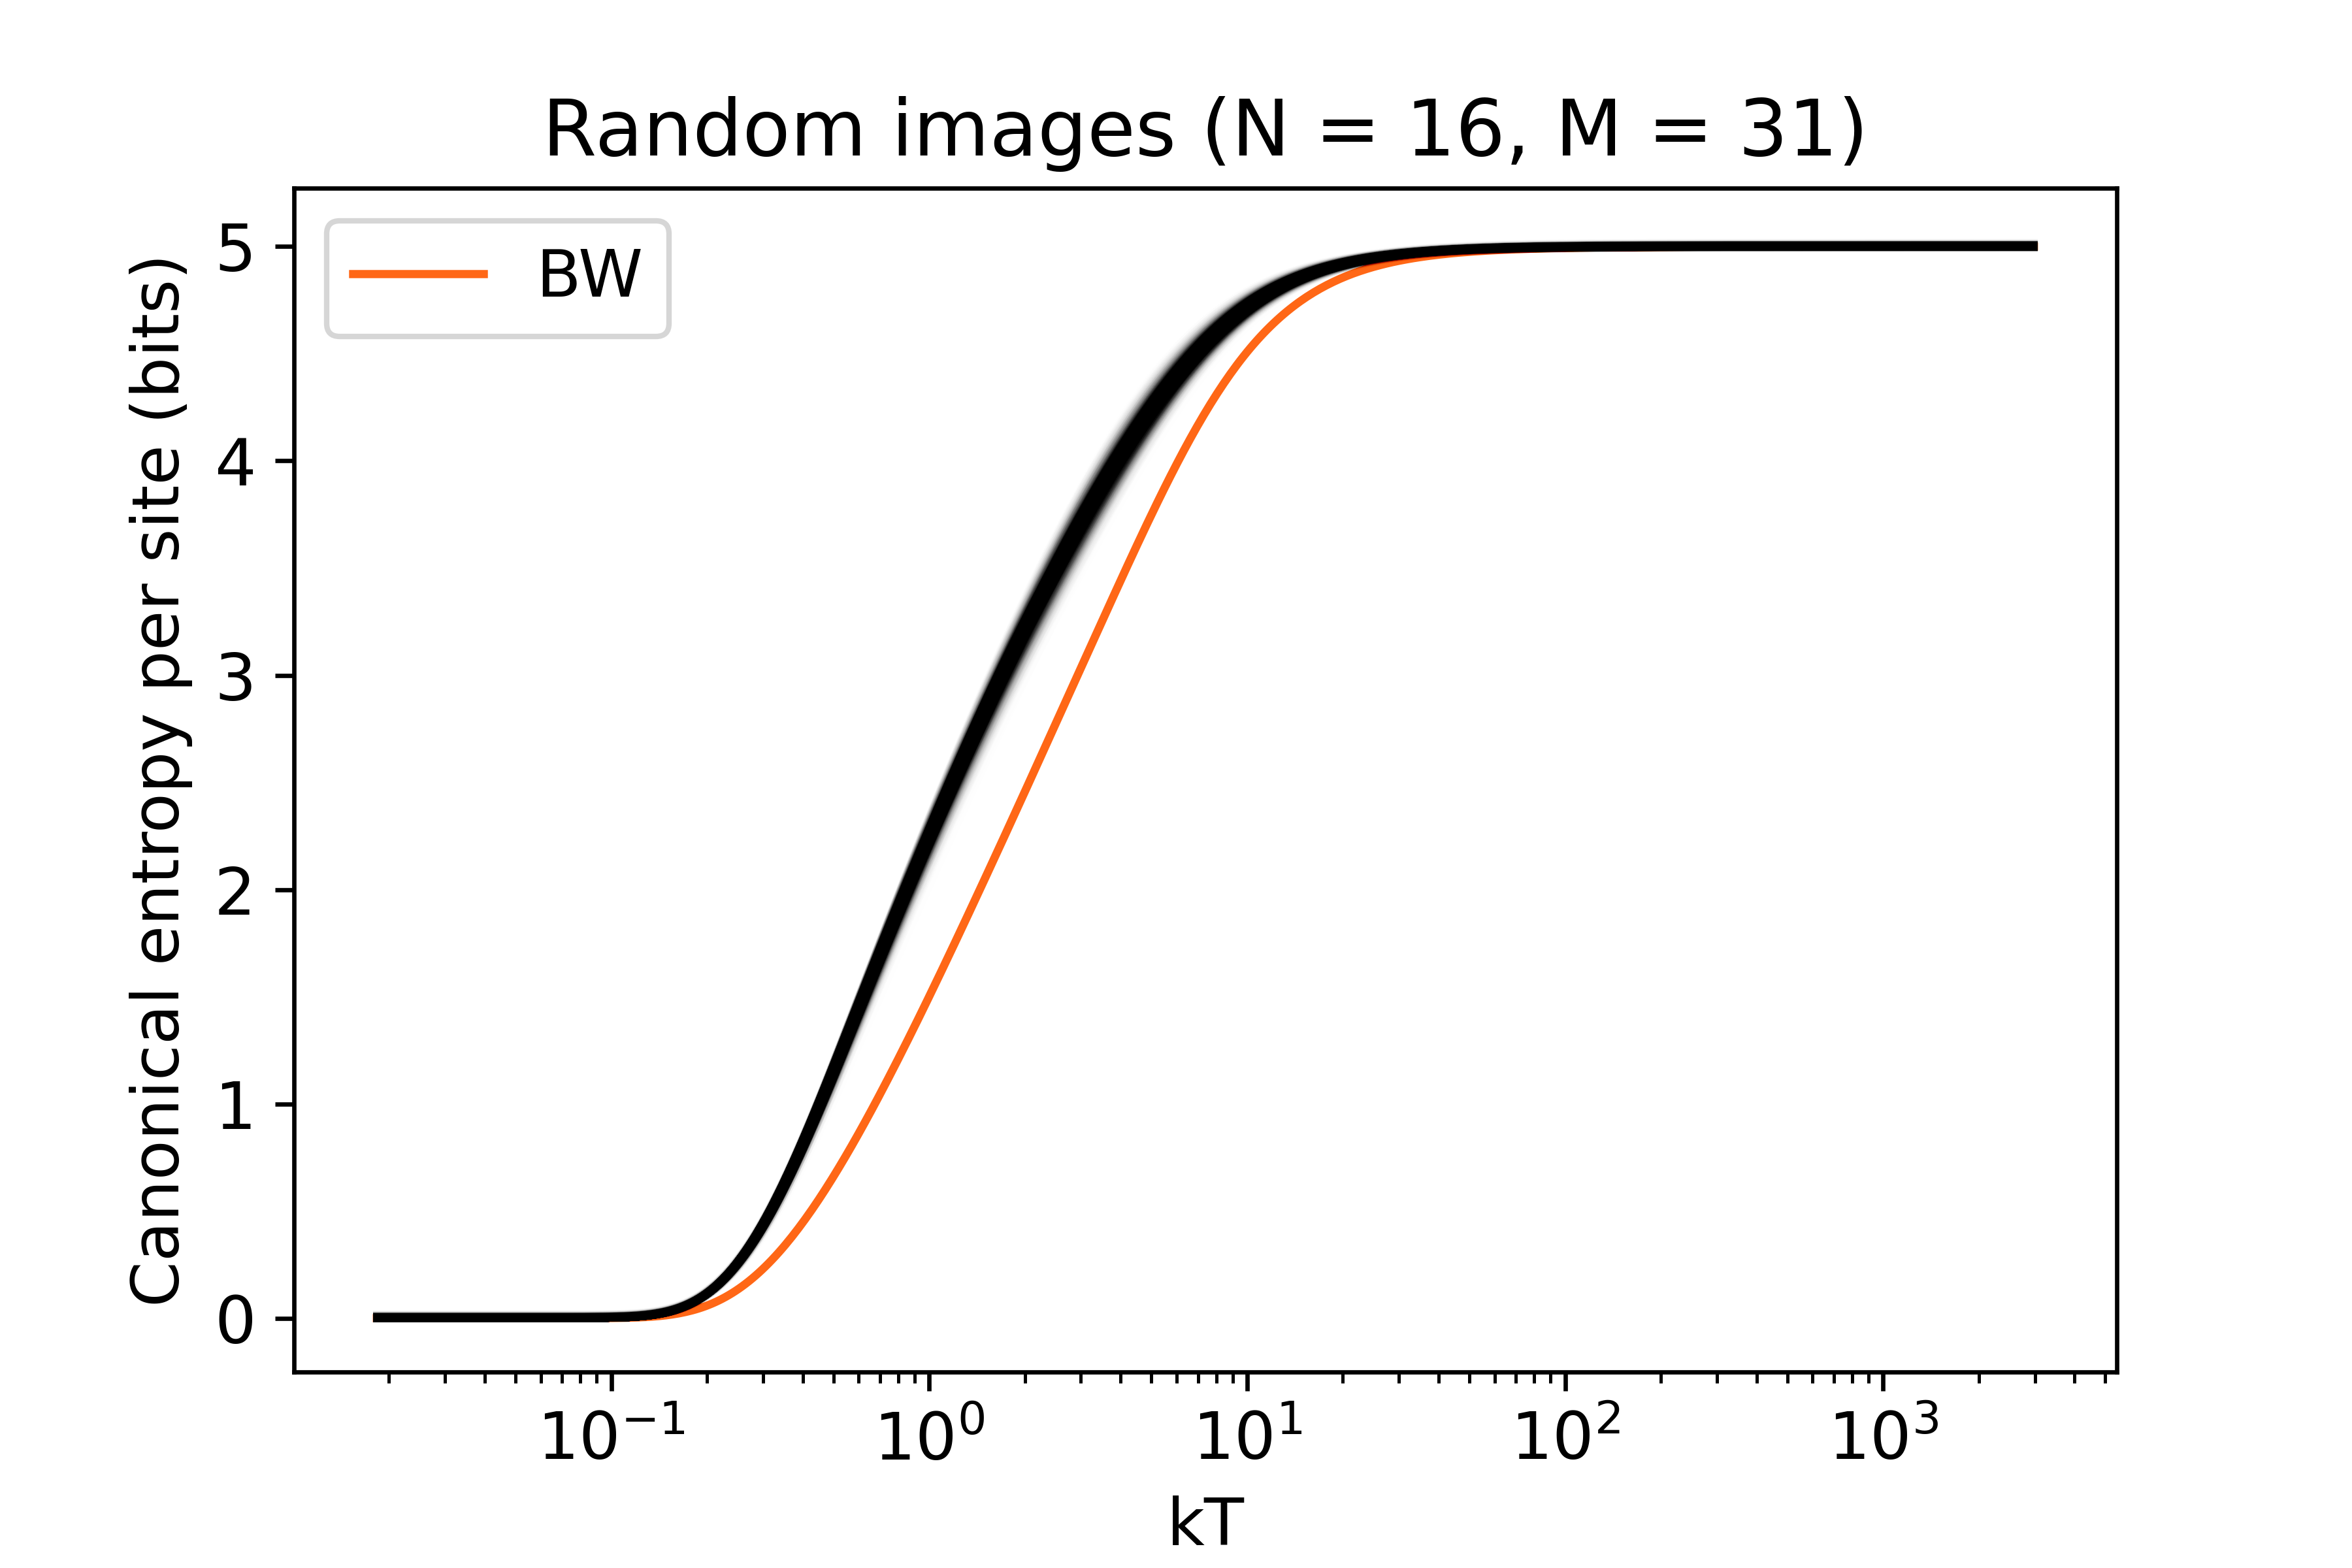
\includegraphics[width=\linewidth]{wanglandau-gray-S}
  \caption{The canonical entropy computed from the simulation density of states for
    \num{1024} random grayscale images. The entropy from the exact result for a
  black image is shown in orange (BW).}\label{fig:wl-gray-S}
\end{figure}

\begin{figure}
  \centering
  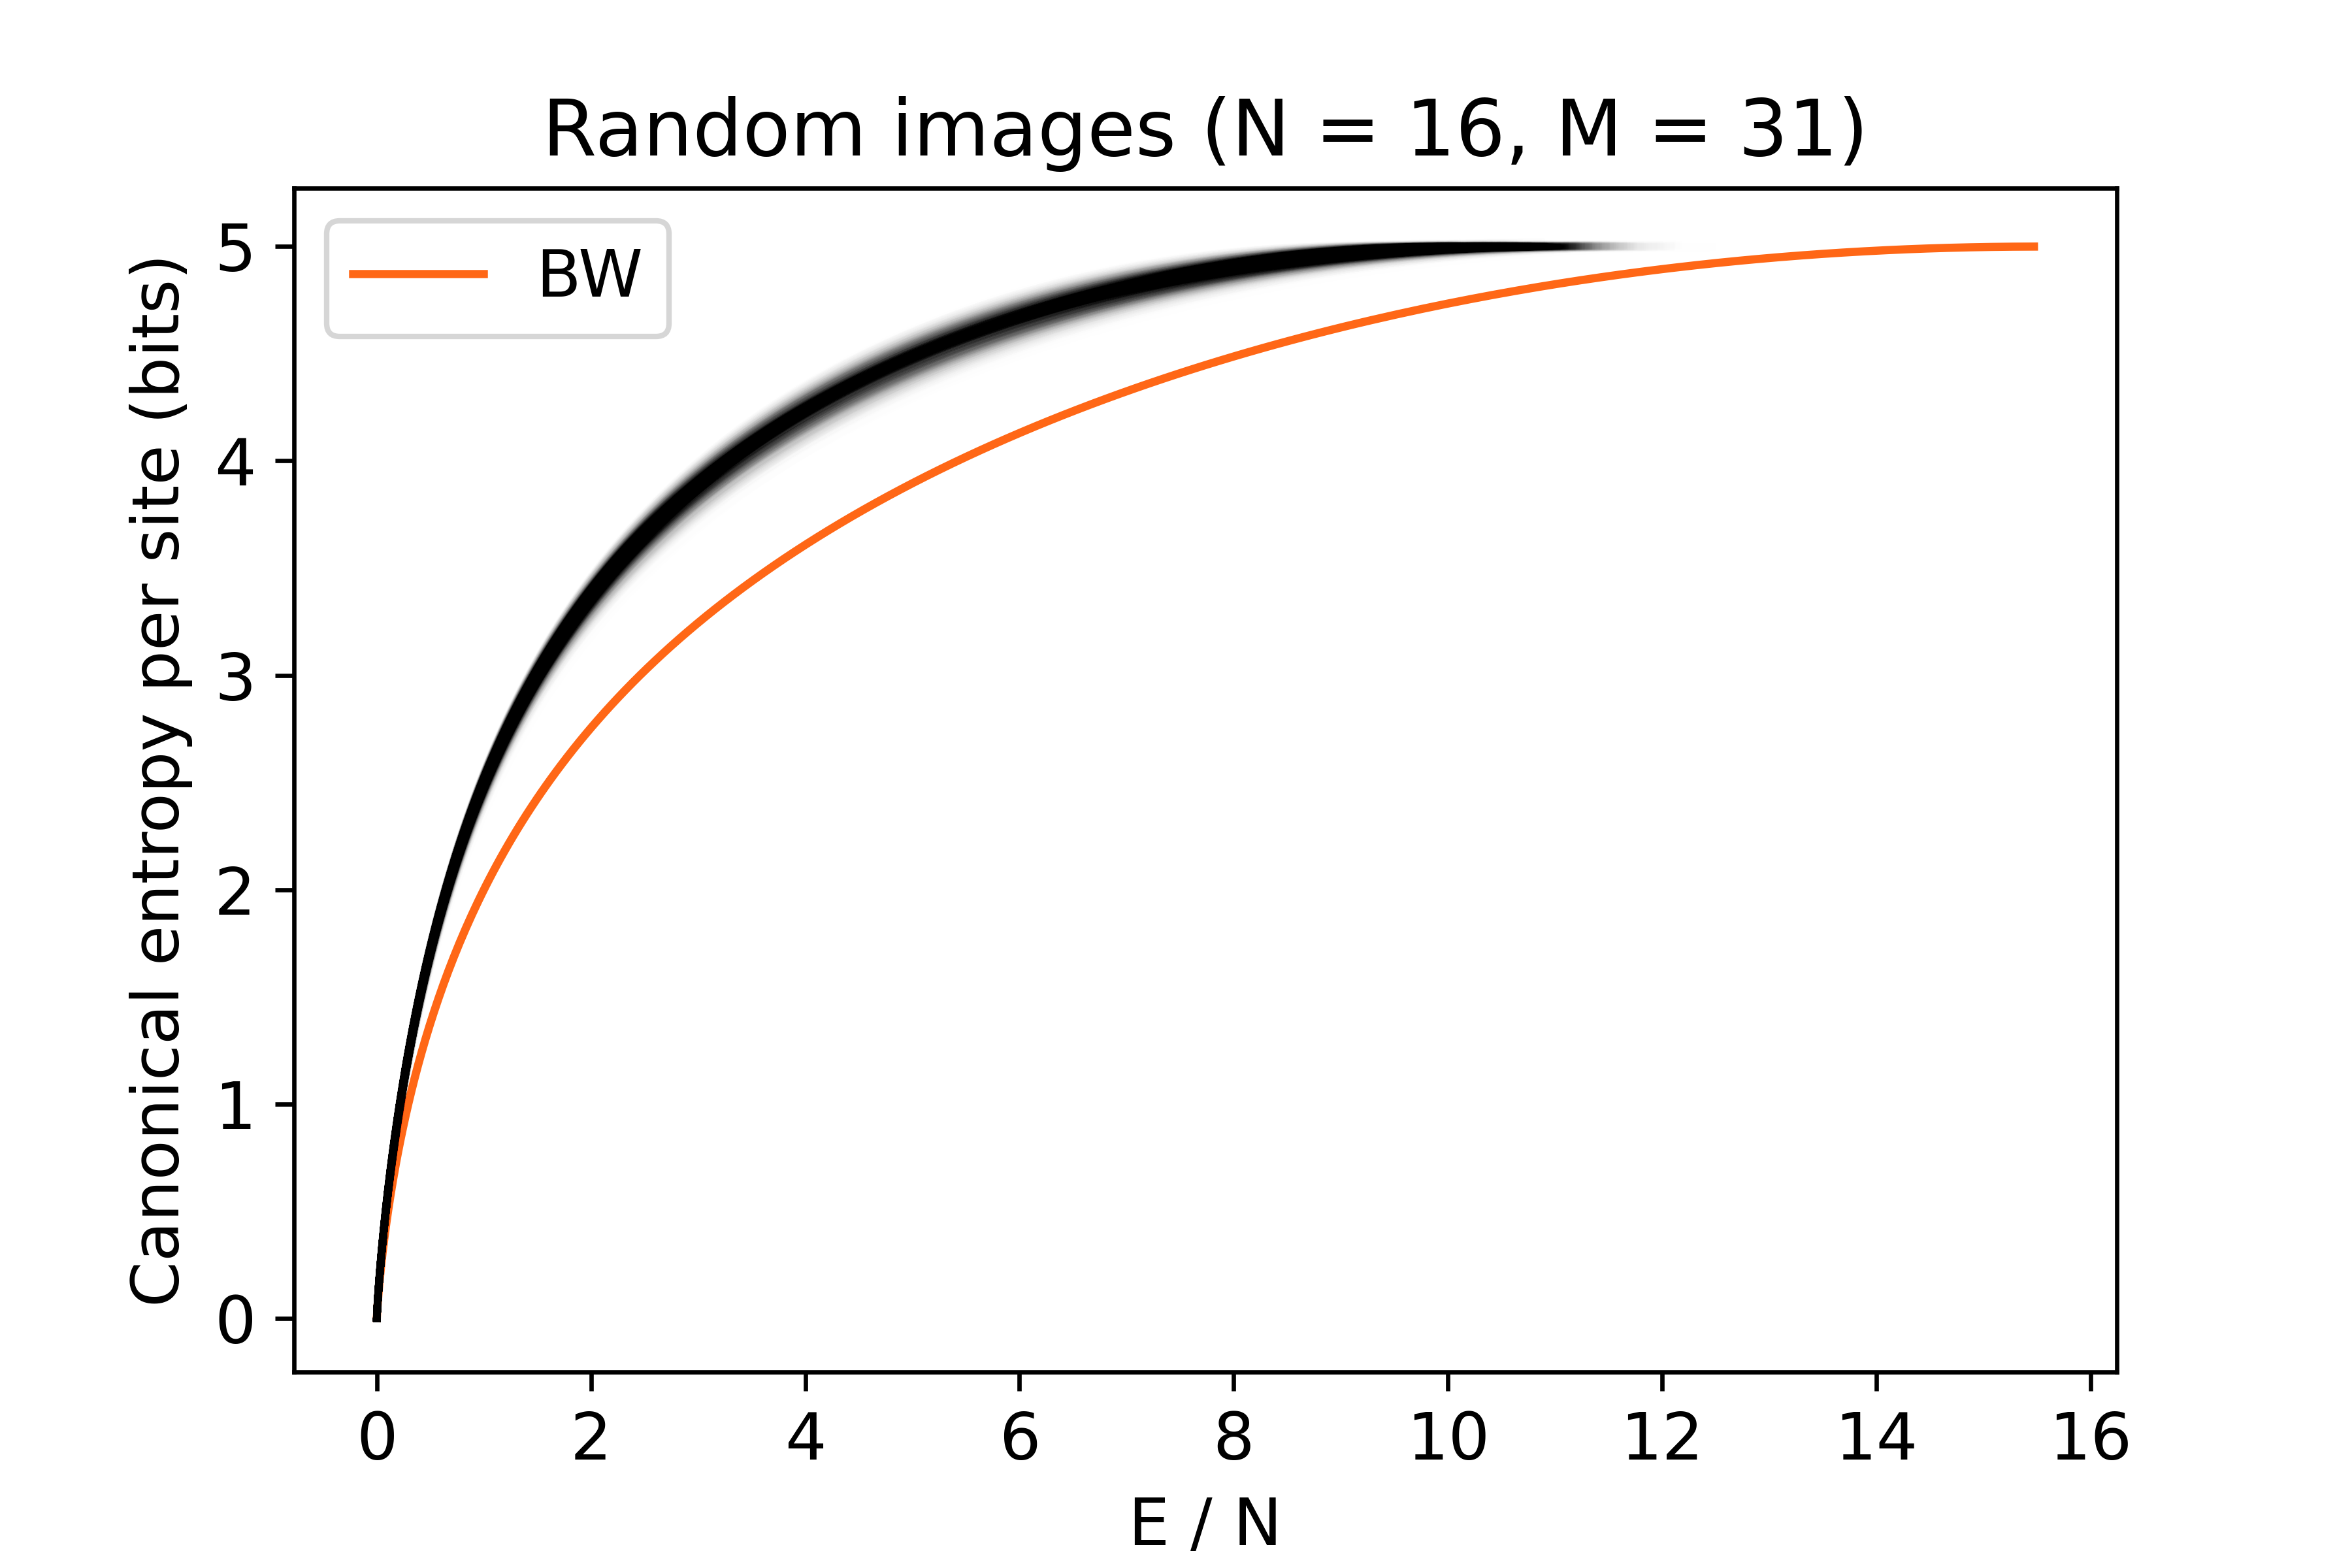
\includegraphics[width=\linewidth]{wanglandau-gray-ES}
  \caption{The canonical entropy for grayscale images increases quickly with
    energy before saturating at the maximum. The entropy from the exact result
  for a black image is shown in orange (BW).}\label{fig:wl-gray-ES}
\end{figure}

The log density of states from WL for a black image is given in
Fig.~\ref{fig:wl-bw}. Since this is indistinguishable from the exact result, we
quantify the error by running \num{1024} simulations for a black image with the
same parameters for histogram flatness and $f$ tolerance as
in~\cite{wanglandau-ajp}. The resulting relative errors are given in
Fig.~\ref{fig:wl-bw-relerror}. This relative error is consistent with that
in~\cite{wanglandau-ajp} for a similarly-sized 2D Ising ferromagnet, which
establishes that the implementation of the algorithm is correct and has the
expected error characteristics.

We now consider the desired calculation of the entropy for random grayscale
images. The WL densities of states for \num{1024} random grayscale images is
given in Fig.~\ref{fig:wl-gray}. The corresponding entropies
(Fig.~\ref{fig:wl-gray-S}) represent the information that we seek. The
entropies for different grayscale images are similar, since the local energy
landscapes for gray pixels are close to the same. The entropy for a black image
is lower than for a grayscale image by almost \SI{1}{bit}, which reflects that
the black pixel values may only fluctuate up in value, rather than in both
directions for a gray pixel value. We may also see how the entropy depends upon
the average energy, which is the quantity we originally considered
(Fig.~\ref{fig:wl-gray-ES}). As expected, this tends towards the log density of
states as the canonical and microcanonical ensembles coincide in the
thermodynamic limit of large $N$ and $M$.

\subsection{Discussion}\label{sec:wl-discussion}

Now that we have computed the modification information as the entropy of a
fluctuating grayscale image, what can we learn from it? If we consider the
fluctuations as noise, we need a psychophysical threshold of the average energy
$E$ where the difference between images is barely noticeable. This is possible,
but requires adjustment of the metric of energy to suit the Weber-Fechner
law~\cite{jnd}. This was not done, since using the absolute
deviation~\eqref{eq:energy} as the energy is simpler to interpret. We may at
least regard the present results as an approximate measure of the information
lost in visual perception.

A limitation of this measure is the use of a digital image instead of
considering the light impinging on the retina as discussed in
Sec.~\ref{sec:vision}. The pixels in an image may be considered as averages of
the true continuous intensity over a small solid angle. Considering a static
grid of pixels in a digital image differs from our foveated imaging process,
which features multiple saccades around a scene to refine points of interest.
This aspect of the issue has previously been addressed by another maximum
entropy method which finds optimally informative fixations based on
contrast~\cite{contrast-entropy}.

Whether the fluctuations are due to noise or varying the scene, the density of
states found in Fig.~\ref{fig:wl-gray} may be used to determine the distribution
of fluctuating values at a single pixel. As indicated by
Fig.~\ref{fig:wl-gray-ES}, even a tiny $4 \times 4$ image has a canonical
entropy similar to the log density of states. Any typical image with thousands
of pixels and hundreds of gray values may be considered in the thermodynamic
limit. In this limit, the distribution of energy for the single pixel $j$ may be
evaluated in the microcanonical ensemble as
\[
  P(E_j \mathbin{|} E)
  = \frac{g(E - E_j;\, N - 1,\, M)}{g(E;\, N,\, M)}
  \approx \frac{g(E - E_j;\, N,\, M)}{g(E;\, N,\, M)}.
\]
For small fluctuations, $E$ is small and $E_j \leq E$ lies on the initial linear
region of the log density of states, no matter the other gray values. Thus,
small fluctuations give rise to an exponential distribution of energies, which
means a Laplacian distribution of gray pixel values. As the total energy $E$
grows towards the maximum density ($T \to \infty$), the Laplacian peak of pixel
values flattens out and increases in entropy.

The final issue is the arbitrary number of values $M$ for the number of gray
values, which affects the entropy value. The simplest solution is to instead
consider the intensive quantity $\flatfrac{S}{\lg M}$, but it is unclear how to
best generalize this to the case of color, where discretizations of different
color spaces may produce different results. This problem of color is avoided in
the case of scotopic (night) vision.

\section{Color and choice of coordinates}\label{sec:color}

The ensemble perspective on images differs from the entropy of statistical
physics in the continuous case. The conjugate nature of position and momentum in
phase space make the thermodynamic differential entropy~\eqref{eq:differential-entropy}
invariant under a canonical coordinate transformation, but this is not so for
color spaces~\cite{diffvar}.

\subsection{Color spaces}

Colors may be represented independently from how they are produced with the
various \emph{\textsc{cie} color spaces}~\cite{cie}. These representations are
ultimately derived from the spectral sensitivities of the different human
\emph{cone cells} which detect colors. The endeavors of the \textsc{cie}
(International Commission on Illumination) have resulted in perceptually-uniform
color spaces like the \textsc{cielab} and \textsc{cieluv} color spaces. Instead
of representing colors as (scaled) \textsc{rgb} values that control hardware
pixels, the \textsc{cie} color spaces use different parameters like the
lightness, chromaticity, and hue coordinates of the \textsc{cielch} space (the
cylindrical version of \textsc{cieluv}). These spaces aim to be scaled so that
the Euclidean distance between the coordinates of two colors captures the
perceptual difference between them. A small enough ball around a color will
contain all colors that are perceptually indistinguishable in the sense of the
just-noticeable difference~\cite{jnd}. This is the kind of perceptual energy
metric that we would like to use in the ensemble perspective, but we are
confronted with the problem of enforcing an arbitrary discretization of the
color space.

\subsection{Choice of coordinates}

Instead of choosing an arbitrary discretization, we propose a relative notion of
information from coordinates which may guide the choice of discretization. As a
motivating example, consider drawing a dot on a ruler. To guess where the dot
is, one would rather know what the ruler reads at the dot location, rather than
the position of the dot along the short side of the ruler. We aim to capture the
sense in which the short side is less informative than the ruled side.

Consider coordinates $x_1,\, \ldots,\, x_m$ for $\RR^m$. An example would be the
spherical coordinates $r,\, \theta,\, \phi$ for $\RR^3$. In terms of probability
distributions, the dot is a distribution which places most of the probability
near a single location. In general, we consider relative coordinate information
for locating points by an arbitrary \emph{target} distribution $p$ on the
coordinates. The usual perspective of independent coordinates as being equally
important is taken as a reference, which we describe with a uniform distribution
$p_u$.
\begin{defn*}
  The \emph{relative information of coordinate $i$} about a target distribution
  $p$ is defined as
  \begin{equation}
    I(x_i)
    = \frac{D_{KL}(p(x_i) \mathbin\| p_u(x_i))}{%
    {D_{KL}(p(x_1,\, \ldots,\, x_m) \mathbin\| p_u(x_1,\, \ldots,\, x_m))}}.
    \label{eq:relinfo}
  \end{equation}
\end{defn*}
We give two simple examples to demonstrate the calculation of the relative
coordinate information.

\subsubsection{Which edge of a ruler is best?}

The different sides of a ruler define Cartesian coordinates on a rectangle. Let
the short side have length $a$ and the ruled side have length $b$. The target
distribution is a uniform distribution on square of side length $c \leq a$
within the ruler. With the coordinates $0 \leq x \leq a$ and $0 \leq y \leq b$,
the uniform reference distribution is $p_u(x,\, y) = {(ab)}^{-1}$ and the target
distribution is $p(x,\, y) = c^{-2} [0 \leq x \leq c,\, 0 \leq y \leq c]$, where
$[P]$ is 1 if $P$ is true and $0$ otherwise. From~\eqref{eq:kl-divergence}
and~\eqref{eq:relinfo} we compute that
\begin{align}
  I(x)
  &= \frac{\log(a/c)}{\log(a/c) + \log(b/c)} \qand \\
  I(y)
  &= \frac{\log(b/c)}{\log(a/c) + \log(b/c)}.
\end{align}
Since the coordinates are independent, $I(x) + I(y) = 1$. We check that the
extreme cases are intuitive. For $c = a$, $I(x) = 0$ and $I(y) = 1$, which is
that all the information is held by the coordinate $y$. This is expected since
the $x$-coordinate is irrelevant for locating a point when $c = a$. As $c \to
0$, $I(x)$ and $I(y)$ tend to $1/2$. In this limit, we see that both coordinates
become equally informative for locating a single point.

\subsubsection{The sphere}

\begin{figure}
  \centering
  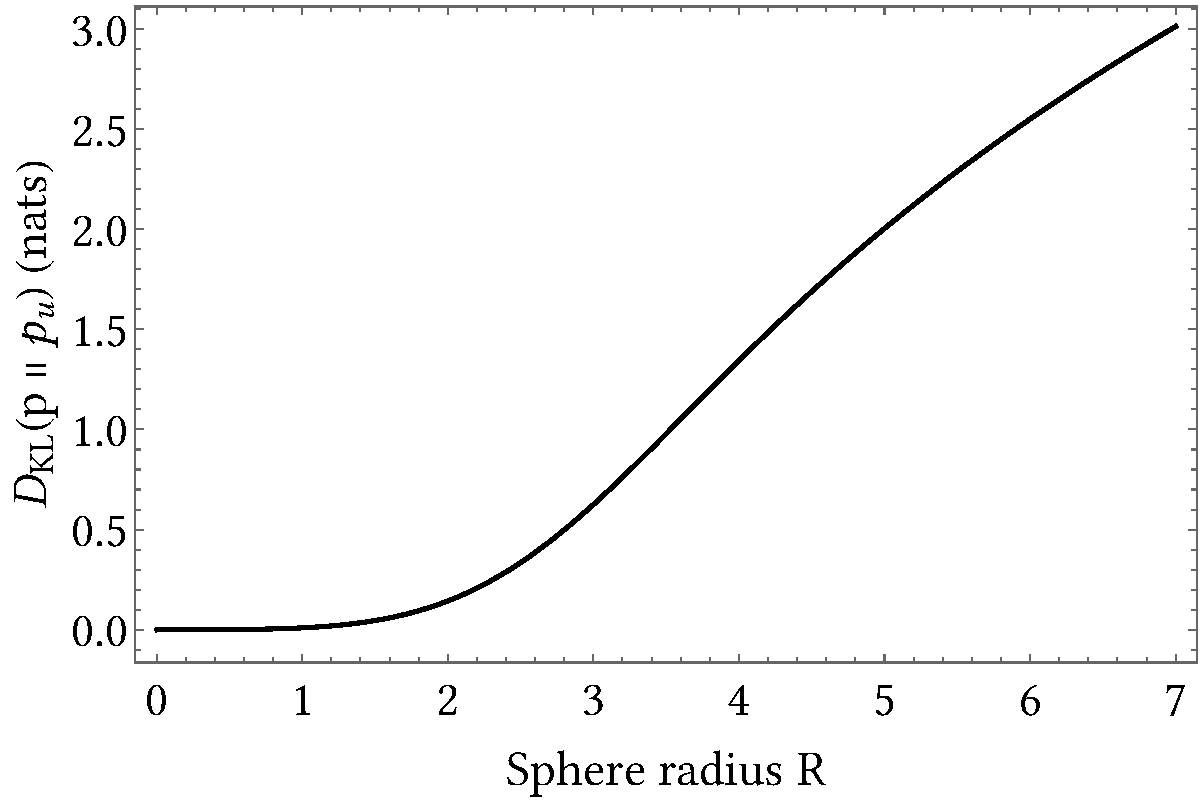
\includegraphics[width=0.8\linewidth]{trunc-norm-ball-kldiv}
  \caption{The KL divergence from uniform to truncated normal as a function of
  ball radius.}\label{fig:trunc-norm-ball-kldiv}
\end{figure}

We may also consider relative coordinate information for coordinate systems with
nontrivial Jacobians, like spherical coordinates. That is, the uniform
distribution on a sphere of radius $R$ in Cartesian coordinates is
\[
  p_u(x,\, y,\, z)
  = \frac{3}{4\pi R^3},
\]
but on spherical coordinates pulls back to
\[
  p_u(r,\, \theta,\, \varphi)
  = \frac{3r^2 \sin\theta}{4\pi R^3}.
\]
The spherical coordinates form independent random variables with marginal
distributions
\[
  p_u(r)
  = \frac{3r^2}{R^3} \qc
  p_u(\theta)
  = \frac{\sin\theta}{2}, \qand
  p_u(\varphi)
  = \frac{1}{2\pi},
\]
whereas the Cartesian coordinates form dependent random variables with
conditional distributions
\[
  p_u(x_i \mathbin{|} x_{j \ne i})
  = \frac{1}{2}{\qty(R^2 - \sum_{j \ne i} x_j^2)}^{-1/2}
  \qq{($i,\, j = 1,\, 2,\, 3$).}
\]
Similarly, the truncated normal distribution with unit variance on the ball
pulls back in spherical coordinates to
\[
  p(r,\, \theta,\, \varphi)
  = {\qty[\mathop{\mathrm{erf}}\qty(\frac{R}{\sqrt{2}})
  - R\sqrt{\frac{2}{\pi}}e^{-R^2 / 2}]}^{-1}
  \frac{e^{-r^2 / 2}}{\sqrt{8\pi^3}}\, r^2 \sin\theta.
\]
We take the truncated normal as our target distribution. While $p(\theta) =
p_u(\theta)$ and $p(\varphi) = p_u(\varphi)$, the marginal distribution of the
radius is
\[
  p(r)
  = {\qty[\mathop{\mathrm{erf}}\qty(\frac{R}{\sqrt{2}})
  - R\sqrt{\frac{2}{\pi}}e^{-R^2 / 2}]}^{-1}
  \frac{e^{-r^2 / 2}}{\sqrt{2\pi}}\, 2r^2.
\]
The KL divergence from the uniform to the truncated normal distribution over the
ball is
\[
  D_{KL}(p \mathbin\| p_u)
  = \int_{r=0}^R \int_{\theta=0}^\pi \int_{\varphi=0}^{2\pi} p \ln
  \frac{p}{p_u} \dd{r}\dd{\theta}\dd{\varphi},
\]
independent of using spherical coordinates
(Fig.~\ref{fig:trunc-norm-ball-kldiv}). But since the spherical coordinates form
independent random variables for both distributions, this separates as
\begin{align}
  D_{KL}(p(r,\, \theta,\, \varphi) \mathbin\| p_u(r,\, \theta,\, \varphi))
  &= D_{KL}(p(r) \mathbin\| p_u(r)) \\
  &+ D_{KL}(p(\theta) \mathbin\| p_u(\theta)) \\
  &+ D_{KL}(p(\varphi) \mathbin\| p_u(\varphi)).
\end{align}
As only the radial distribution is different,
\[
  D_{KL}(p(r,\, \theta,\, \varphi) \mathbin\| p_u(r,\, \theta,\, \varphi))
  = D_{KL}(p(r) \mathbin\| p_u(r)),
\]
as expected from the symmetries. Thus $I(r) = 1$ and $I(\theta) = I(\phi) = 0$.
This is consistent with the intuition that the radius alone controls the
probability of a point. Put negatively, knowing angles $\theta$ and $\phi$ for a
point gives no information about if it is probable.

\subsubsection{Relevance to color spaces}

We have now set up the machinery to compare different coordinates on color
spaces. Future work could assess the probability distribution on a color space
from natural images, as in~\cite{natstat-color}, or consider the visible gamut
of colors as a uniform distribution over a subset of a \textsc{cie} color space.
A computation of relative coordinate information for a color space with one of
these two target distributions would indicate which coordinates of the color
space are perceptually important. For example, we might expect that luminance
would be important, given the importance of identifying edge contrast in vision.
The target distributions could also be used to find an optimal entropy coding
which would reduce the information needed to express natural colors.

\section{Conclusion}

The idea of visual complexity has been explored through conventional
perspectives rooted in natural image statistics, as well as through the new
perspectives from an image ensemble and relative coordinate information. These
notions of visual complexity have varied applications to disciplines like
computer vision, compressive sensing, image compression, and computer graphics.
Taken together, the different perspectives that we have discussed model much of
the visual complexity in the natural world in much the same way that the simple
harmonic oscillator acts as a model for natural phenomena like bobbing in water
or the swaying of trees.

While we have largely considered images as entities in their own right, it
should be noted that their visual complexity is rooted in the complex phenomena
of the natural world. Many of the ideas covered here are relevant to
understanding the complexity of physical laws as well as vision. Thought in
physics along these lines may be found in proceedings of the Santa Fe
Institute~\cite{santa-fe} or in P.\ W.\ Anderson's maxim that ``more is
different''~\cite{anderson}. We may only hope that the enrichment to
applications in vision embodied by the success of image compression algorithms
and computer rendering due to understanding visual complexity has an analog in
physics and other natural sciences.

\section{Acknowledgements}

Most of all, I thank Prof.\ Vincent Meunier for proposing and mentoring the
project. Our near-daily meetings became highlights of the long days spent inside
during the summer of \textsc{covid-19}. I also thank Profs. Peter Persans and K.
V. Lakshmi for all their effort in coordinating an unusual physics \textsc{reu}.
Funding for this project was provided as a part of the physics research
experience for undergraduates program of the National Science Foundation at
Rensselaer Polytechnic Institute.

\appendix

\section{Theorems}

\begin{thm}\label{thm:self-information}
  The only twice continuously differentiable function $I(x)$ that satisfies the
  axioms in Sec.~\ref{sec:information-theory} is the self-information $I(x) =
  -\log p(x)$.
  \begin{proof}
    Consider independent events $x$ and $y$ with probabilities $p$ and $p'$. The
    axioms only concern the probabilities of the events, so we may express the
    information as $I(x) = \tilde{I}(p(x))$. Then as proposed,
    \[
      I(x,\, y)
      = \tilde{I}(pp')
      = \tilde{I}(p) + \tilde{I}(p')
    \]
    by independence. Taking the partial derivative with respect to $p$ gives
    \[
      p' \tilde{I}'(pp')
      = \tilde{I}'(p),
    \]
    and then taking the partial derivative with respect to $p'$ gives
    \[
      \tilde{I}'(pp') + pp' \tilde{I}''(pp')
      = 0.
    \]
    We may then define $q = pp'$ to obtain the differential equation
    \[
      \dv{q}\qty(q \tilde{I}'(q))
      = 0,
    \]
    which has solution
    \[
      \tilde{I}(q) = k\log q
    \]
    for real $k$. The condition that $\tilde{I}(q) \ge 0$ requires $k > 0$,
    which is equivalent to a choice of base for the logarithm.
  \end{proof}
\end{thm}

\begin{thm}\label{thm:bw-g}
  The number of tuples $(a_1,\, \ldots,\, a_N)$ with $0 \leq a_i \leq M - 1$ and
  $\sum_i a_i = E$ is
  \[
    g(E)
    = \sum_k {(-1)}^k \binom{N}{k} \binom{N + E - Mk - 1}{E - Mk}.
  \]
  \begin{proof}
    Ordinary generating functions provide the solution~\cite{genfunc}. We represent the sum $E$
    as the exponent of a integer polynomial in $z$ in the following way. For the
    tuple $(x_1,\, x_2)$, we represent $x_1$ as $z^{x_1}$ and $x_2$ as
    $z^{x_2}$. Together, we have $z^{x_1} z^{x_2}$, which gives the monomial
    $z^{x_1 + x_2} = z^E$ for this tuple. We may then find $g(E)$ as the
    coefficient of $z^E$ in
    \[
      {\qty(1 + \cdots + z^{M-1})}^N.
    \]
    Expanding using the binomial theorem gives
    \begin{align}
      {\qty(\frac{1 - z^M}{1 - z})}^N
      &= \sum_{k=0}^N {(-1)}^k \binom{N}{k} z^{Mk}
      \sum_{j=0}^\infty {(-1)}^j \binom{-N}{j} z^j \\
      &= \sum_{k=0}^N \sum_{j=0}^\infty {(-1)}^k \binom{N}{k}
      \binom{N + j - 1}{j} z^{Mk + j}.
    \end{align}
    The value of $j$ for $z$ to have exponent $E$ is $j = E - Mk$, so the
    coefficient of $z^E$ in the polynomial is
    \begin{equation}
      g(E)
      = \sum_k {(-1)}^k \binom{N}{k} \binom{N + E - Mk - 1}{E - Mk},
    \end{equation}
    where the limits of summation are set by the binomial coefficients.
  \end{proof}
\end{thm}

\section{Wang-Landau algorithm implementation}\label{sec:wanglandau-core}

The relevant core of the Wang-Landau algorithm implementation is reproduced
below. For the full code, see the \textsc{reu} project
repository~\cite{rpi-reu-notebook}, which includes both the code and a notebook
of all progress, including some other approaches to visual complexity than those
described in this report.

\inputminted{python}{wanglandau-core.py}

\hypersetup{urlcolor=Mahogany}
\bibliography{references}

\end{document}

